


In this section, we present the experimental evaluations. All the experiments are designed to answer the following two questions:

\begin{itemize}
	\item {\bf Q1. Effectiveness.} How effective are the proposed reasoning methods, including both pairwise and collective comparative reasoning methods?
	\item {\bf Q2. Efficiency.} How fast are the proposed methods? %The effectiveness of pair-wise comparative reasoning and collective comparative reasoning.
\end{itemize}


Two data graphs are used in the experiments: Yago ~\cite{yago} \footnote{It is publicly available at \url{https://www.mpi-inf.mpg.de/de/departments/databases-and-information-systems/research/yago-naga/yago/downloads}. We use the core version.} and Covid-19 \footnote{The dataset can be found at \url{http://blender.cs.illinois.edu/covid19/}. }.
Yago ~\cite{yago} is a widely used knowledge graph which contains 12,430,705 triples, 4,295,825 entities and 39 predicates.
The Covid-19 data graph contains three types of entities which are {\tt Gene}, {\tt Disease} and {\tt Chemical}.
In our experiments, we use a subset of the Covid-19 dataset which contains 55,434 core entities and 5,527,628 triples.
We compare our method with 4 baselines, including:

\begin{itemize}
    \item TransE ~\cite{transE} embeds both the entities and relations in the knowledge graph to a high dimension embedding space, and checks the consistency of a triple according to the embedding distance.
    \item Jaccard coefficient ~\cite{jaccard} is a link prediction algorithm which measures the truthfulness of the triple according to the number of common neighbor nodes of the head entity and tail entity.
    \item Knowledge Linker ~\cite{KL}, short for KL, extracts a path between the head entity and tail entity to decide whether the input triple is correct.
    \item KGMiner ~\cite{kgminer} extracts a subgraph between the head entity and tail entity to predict the truthfulness of the input clue.
    %\item KomPare ~\cite{kompare} leverages graph kernel to find important elements inside knowledge segments and make decision according to these important elements.
\end{itemize}

All the experiments are conducted on a moderate desktop with an Intel Core-i7 3.00GHz CPU and 64GB memory.
The source code could be found at \url{https://github.com/lihuiliullh/KompaRe}.
For TransE ~\cite{transE} in the experiments, we set the embedding dimension to 64 and use a margin of one and a learning rate of 0.01 for 1,200 epochs.










\subsection{Predicate-Predicate Similarity Efficacy}

\begin{figure}[ht]
\centering
	\begin{subfigure}[exports]{
		\centering
		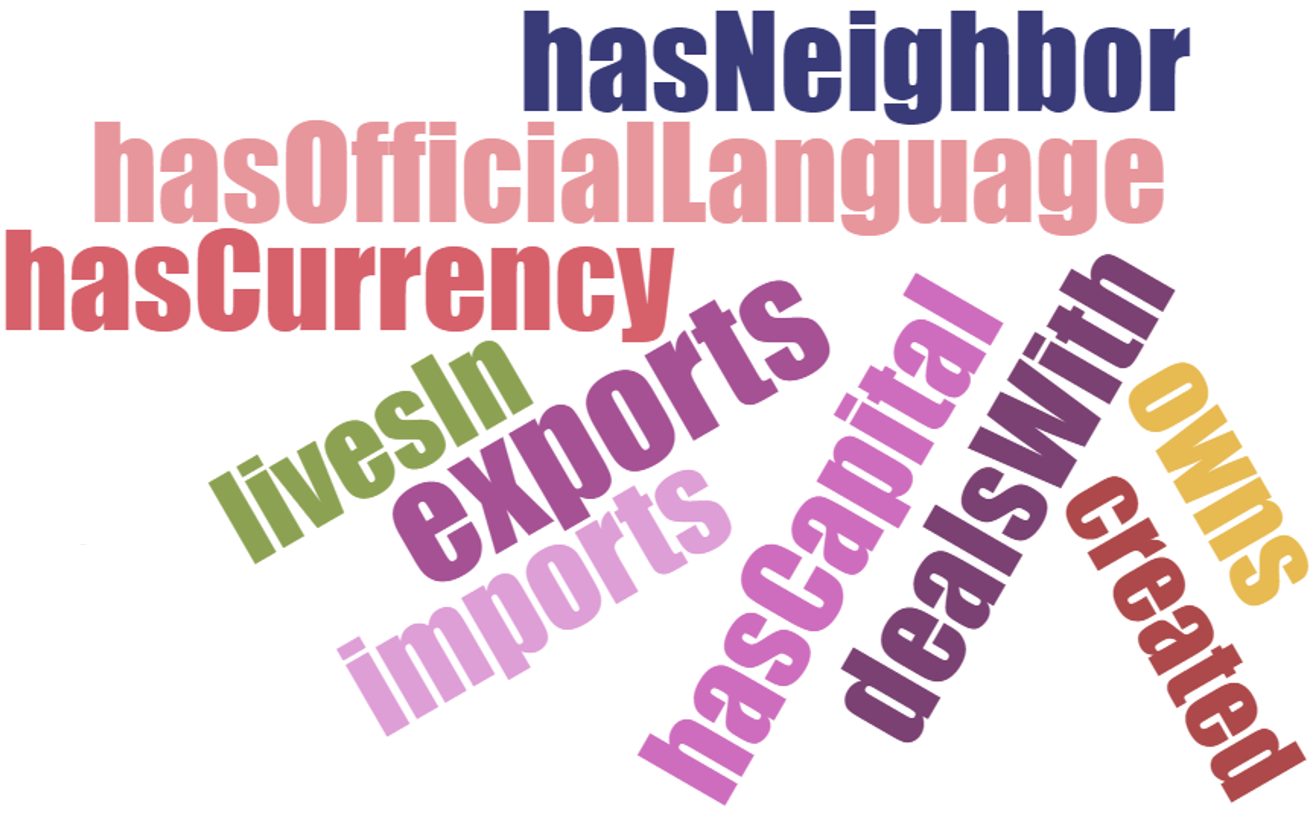
\includegraphics[width=0.35\textwidth]{submissions/logical-queries-uiuc/img/export.png}
		\label{subfig:dbqa}}
	\end{subfigure}
	\begin{subfigure}[livesIn]{
		\centering
		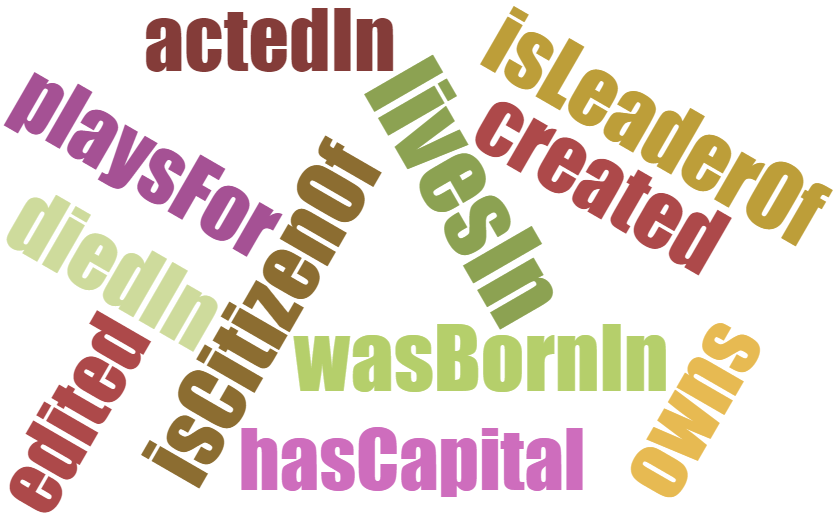
\includegraphics[width=0.35\textwidth]{submissions/logical-queries-uiuc/img/livesIn.png}
		\label{subfig:dbqa}}
	\end{subfigure}
%  \subfloat[exports]{
%	\begin{minipage}[c][0.5\width]{
%	   0.35\textwidth}
%	   \centering
%	   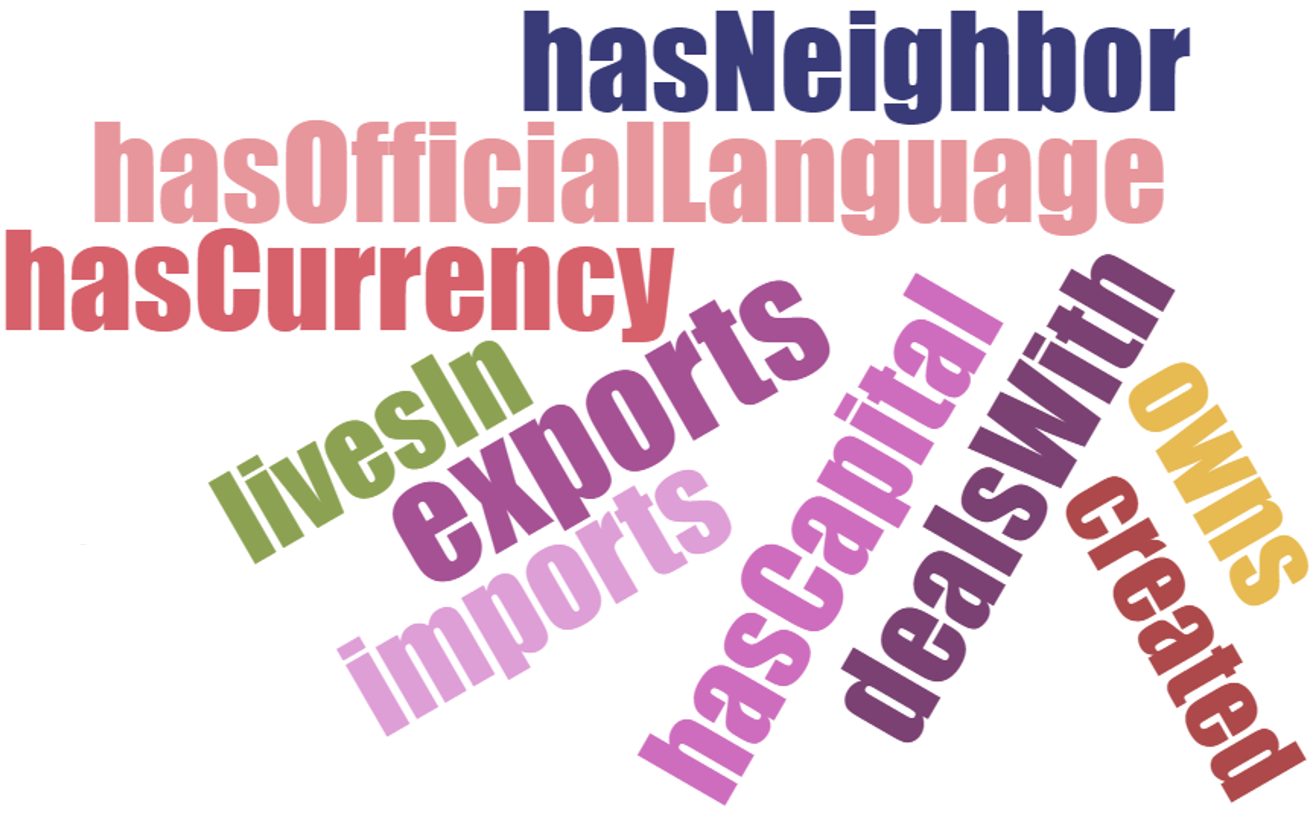
\includegraphics[width=1\textwidth]{submissions/logical-queries-uiuc/img/export.png}
%	\end{minipage}}
%%  \hfill 	
%\hspace{0.1\textwidth}
%  \subfloat[livesIn]{
%	\begin{minipage}[c][0.5\width]{
%	   0.35\textwidth}
%	   \centering
%	   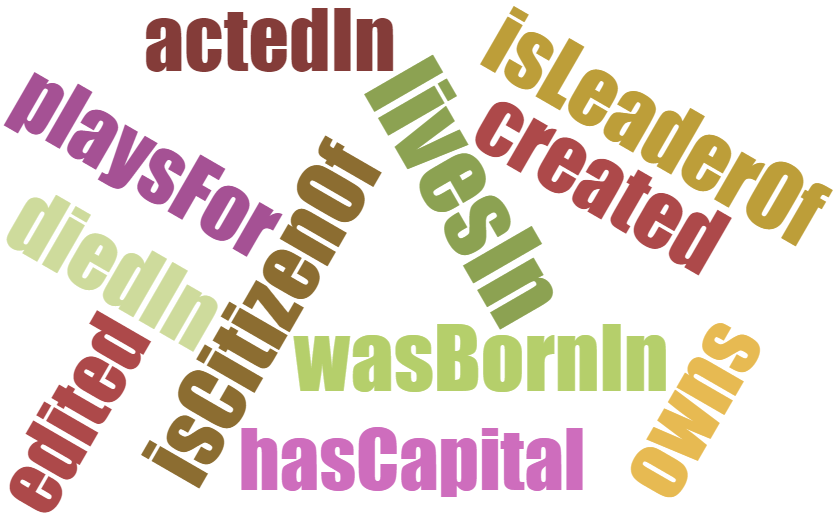
\includegraphics[width=1\textwidth]{submissions/logical-queries-uiuc/img/livesIn.png}
%	\end{minipage}}
\caption{Top-{\em 10} most similar predicates in Yago.}
\label{word-cloud}
\end{figure}

We evaluate the proposed predicate-predicate similarity. Figure ~\ref{word-cloud} presents two examples on Yago dataset. It shows the top-{\em 10} most similar predicates with {\tt exports} and {\tt livesIn}, respectively. The font size in Figure~\ref{word-cloud} is proportional to the predicate-predicate similarity value.
The top similar predicates w.r.t. {\tt exports} by our method include {\tt imports}, {\tt hasOfficialLanguage}, {\tt dealsWith}, all of which have a high similarity with {\tt exports}. They all provide specific semantic information about {\tt exports}.
Likewise, the top similar predicates w.r.t. {\tt livesIn} include {\tt wasBornIn}, {\tt isCitizenOf}, {\tt diedIn}, all of which are closely related to {\tt livesIn}. %They all talk about information related to some places or countries.
These results showcase that the proposed TF-IDF based method can effectively measure the similarity between different predicates.

Table ~\ref{appendix-pred-sim} shows the predicate similarity between {\tt isTypeOf} and other predicates. %We only list the predicates we used in this paper.
\begin{table}[!htbp]
    \centering
    \scriptsize
    \caption{Predicate similarity of {\tt isTypeOf} with others}
    \vspace{-1\baselineskip}
    \begin{tabular}{ |c|c|c|c|c|c|c|c| }
  \hline
  predicate & sim & predicate & sim & predicate & sim & predicate & sim \\
  \hline
 isCitizenOf &  0.840 &  isLeaderOf &  0.955 & isAffiliatedTo &  0.808 &  isPoliticianOf &  0.917 \\
 livesIn &  0.972 &  owns &  0.945 & exports &  0.706 &  dealsWith &  0.697\\
 hasCapital &  0.786 &  command &  0.216 & happenedIn &  0.767 &  participatedIn &  0.869\\
 worksAt &  0.752 &  isLocatedIn &  0.870 & & & &\\
  \hline
\end{tabular}
\label{appendix-pred-sim}
\end{table}


\vspace{-1.0\baselineskip}
\subsection{Pair-wise Comparative Reasoning}\label{exp-pair-section}

\begin{table*}
	\centering
	\caption{Accuracy of pair-wise comparative reasoning.
	}
	\scriptsize
	\vspace{-1\baselineskip}
	\setlength\tabcolsep{1.5pt}
	\begin{tabular}{|c|c|c|c|c|c|c|c|c|c|c|c|c|}
	\hline
	Dataset       & \makecell{\# of \\ queries}   & TransE & Jaccard  & KL  & KGMiner & Neural Network Based & Graph Kernel Based \\ \hline
	\makecell{Family members positive}   & 300  & 0.682 & 0.831 & 0.618 & {0.983} & \textbf{1.000} & 0.944 \\ \hline
	\makecell{Family members negative}   & 300  & 0.335 & 0.169 & \textbf{1.000} & \textbf{1.000} & 0.000 & 0.941 \\ \hline
    \makecell{Graduated college positive} & 300  & 0.686 & 0.335 & 0.502 & 0.769 &  \textbf{0.879} & {0.794} \\ \hline
    \makecell{Graduated college negative} & 300  & 0.626 & 0.993 & 0.947 & 0.901 & 0.367 & \textbf{0.994} \\ \hline
    \makecell{Live place positive}     & 300    & 0.567 & 0.415 & 0.489 & \textbf{0.834} & 0.086 & 0.762 \\ \hline
    \makecell{Live place negative}    & 300    & 0.802 & 0.585 & \textbf{0.907} & 0.900 & 0.732 & 0.888 \\ \hline
    \makecell{Birth place positive}    & 300    & 0.590 & 0.435 & 0.537 & 0.698 & 0.656 & \textbf{0.800} \\ \hline
    \makecell{Birth place negative}    & 300    & 0.845 & \textbf{1.000} & 0.973 & 0.927 & 0.719 & 0.927 \\ \hline
    \makecell{Work place positive}     & 300    & \textbf{0.751} & 0.319 & 0.445 & 0.698 & 0.700 & {0.720} \\ \hline
    \makecell{Work place negative}     & 300    & 0.624 & 0.994 & 0.942 & 0.927 & 0.803 & \textbf{0.995} \\ \hline
    $mean \pm std$  & - & 0.651 $\pm$ 0.424 & 0.608 $\pm$ 0.302 & 0.736 $\pm$ 0.221 & 0.864 $\pm$ 0.105 & 0.594 $\pm$ 0.333 & \textbf{0.877 $\pm$ 0.095}  \\ \hline
	\end{tabular}
\label{pair_dataset}
\end{table*}
Here, we evaluate the effectiveness of the proposed pair-wise comparative reasoning.
Ten query sets are used in the experiments.
For each positive query set, it contains a set of queries which describe the true claim, while for each negative query set, it contains a set of queries which describe the false claim. For example, in query set ``Birth Place", $<${\tt Alan Turing}, {\tt wasBornIn}, {\tt Maida Vale}$>$ and $<${\tt Alan Turing}, {\tt wasBornIn}, {\tt United Kingdom}$>$ is a positive query pair, while $<${\tt Alan Turing}, {\tt wasBornIn}, {\tt Maida Vale}$>$ and $<${\tt Alan Turing}, {\tt wasBornIn}, {\tt Canada}$>$ is an negative query pair.
The positive queries are generated by sampling some true claims in the knowledge graph. The negative queries are generated by substituting one subject of the positive queries.
The accuracy is defined as $\frac{N}{M}$ where $N$ is the number of queries correctly classified by pair-wise comparative reasoning and $M$ is the total number of queries.
When checking the consistency of a query pair $<{\tt s_1}, {\tt p_1}, {\tt o_1}>$ and $<{\tt s_2}, {\tt p_2}, {\tt o_2}>$,
because none of the baseline methods is designed for pair-wise comparative reasoning, we use them to check each triple in the pair, if any triple is classified as false, this query pair is treated as false. Otherwise, we further check the
truthness of $<{\tt o_1}, {\tt isTypeOf}, {\tt o_2}>$ and $<{\tt o_2}, {\tt isTypeOf}, {\tt o_1}>$,
if one of them is classified as consistency, this query pair is treated as consistency.
Table ~\ref{pair_dataset} gives the detailed results.


As we can see, Graph Kernel based method and KGMiner ~\cite{kgminer} have the highest accuracy most of the time. But Graph Kernel based method has the highest average accuracy and the lowest variance compared with other methods.

\subsection{Neural Network Based Pair-wise Comparative Reasoning}
We conduct more experiments in this section to test the effectiveness of Neural Network Based Pairwise comparative reasoning.
Six binary classifiers are used in the experiment. Table ~\ref{pair_dataset_bin_3} shows the details of each classifier and their performance on different query sets.
As we can see, different methods have different performances. Logistic Regression has the highest average accuracy and K-Nearest Neighbor has the highest average recall.


\begin{table}[!htbp]
\begin{adjustwidth}{-.5in}{-.5in}
        \begin{center}
    \centering
	\caption{Accuracy, recall and precision of neural network based pair-wise comparative reasoning
	}
	\scriptsize
	\vspace{-1\baselineskip}
	\setlength\tabcolsep{1.5pt}
	\begin{center}
	\begin{tabular}{|c|c|c|c|c|c|c|c|c|c|c|c|c|c|c|c|c|c|c|}
	\hline
	
 \diagbox{Model}{Dataset} & \multicolumn{3}{c|}{Family members} & \multicolumn{3}{c|}{Graduated college}& \multicolumn{3}{c|}{Live place}&\multicolumn{3}{c|}{Birth place}& \multicolumn{3}{c|}{Work place}& \multicolumn{3}{c|}{$mean \pm std$ }\\\hline

  measurements  & Acc & Prec & Recall & Acc & Prec & Recall &Acc & Prec & Recall &Acc & Prec & Recall &Acc & Prec & Recall &Acc & Prec & Recall\\
    \hline


% 	 &\makecell{family members}&\makecell{family members}&\makecell{family members} &\makecell{family members}&\makecell{family members} &\makecell{family members} \\ \hline
% 	 \multicolumn{1}{|c|}{messurements}  & Acc & Prec & Recall & Acc & Prec & Recall& Acc & Prec & Recall& Acc & Prec & Recall& Acc & Prec & Recall& Acc & Prec & Recall\\\hline
	\# of  queries &  \multicolumn{3}{c|}{506} & \multicolumn{3}{c|}{499} & \multicolumn{3}{c|}{560} & \multicolumn{3}{c|}{470} & \multicolumn{3}{c|}{540} & \multicolumn{3}{c|}{-} \\ \Xhline{1.5pt}
% 	Logistic Regression   &.682 & 0.831 & 0.618 & {0.983} \\ \hline
%     Support Vector Machines  & 0.686 & 0.335 & 0.502 & 0.769  \\ \hline
%     Decision Trees          & 0.567 & 0.415 & 0.489 &090\\ \hline
%     Random Forest      & 0.590 & 0.435 & 0.537 & 0.698  \\ \hline
%     Naive Bayes         & \textbf{0.751} & 0.319 & 0.445 & 0.698 \\ \hline
%     K-Nearest Neighbor      & \textbf{0.751} & 0.319 & 0.445 & 0.698 \\ \hline
Logistic Regression & 0.480 & 0.519 & 0.491 & 0.693 & 0.660 & 0.729 & 0.619 & 0.732 & 0.594 & 0.674 & 0.816 & 0.645 & 0.743 & 0.786 & 0.733 & \textbf{0.642}$\pm$\textbf{0.090} & 0.703$\pm$0.106 & 0.639$\pm$0.091 \\ \hline
SVM & 0.431 & 0.154 & 0.364 & 0.416 & 0.113 & 0.333 & 0.611 & 0.768 & 0.581 & 0.516 & 1.000 & 0.516 & 0.688 & 0.911 & 0.637 & 0.532$\pm$0.104 & 0.589$\pm$0.380 & 0.486$\pm$0.119 \\ \hline
Decision Trees & 0.422 & 0.519 & 0.443 & 0.713 & 0.623 & 0.786 & 0.619 & 0.696 & 0.600 & 0.611 & 0.694 & 0.607 & 0.716 & 0.750 & 0.712 & 0.616$\pm$0.107 & 0.656$\pm$\textbf{0.080} & 0.629$\pm$0.116 \\ \hline
Random Forest & 0.314 & 0.462 & 0.364 & 0.624 & 0.528 & 0.683 & 0.673 & 0.714 & 0.656 & 0.684 & 0.673 & 0.702 & 0.706 & 0.661 & 0.740 & 0.600$\pm$0.146 & 0.608$\pm$0.096 & 0.629$\pm$0.135 \\ \hline
Naive Bayes & 0.461 & 0.615 & 0.478 & 0.624 & 0.830 & 0.603 & 0.522 & 0.839 & 0.511 & 0.632 & 0.878 & 0.597 & 0.725 & 0.911 & 0.671 & 0.593$\pm$0.092 & \textbf{0.815}$\pm$0.104 & 0.572$\pm$\textbf{0.069} \\ \hline
K-Nearest Neighbor & 0.392 & 0.500 & 0.419 & 0.683 & 0.774 & 0.672 & 0.646 & 0.589 & 0.660 & 0.695 & 0.673 & 0.717 & 0.761 & 0.821 & 0.742 & 0.636$\pm$0.127 & 0.672$\pm$0.118 & \textbf{0.642}$\pm$0.115 \\ \hline
	\end{tabular}
\end{center}
\label{pair_dataset_bin_3}
\end{center}
    \end{adjustwidth}
\end{table}

Table ~\ref{pair_dataset_bin_Acc} shows performance of the neural network based method on each positive and negative query dataset. Based on the results in the table, we can conclude that the accuracy of the neural network based model is lower than that of other models, e.g., KGMiner and Graph Kernel Based method.

\begin{table}[!htbp]
	\centering
	\caption{Accuracy of neural network based pair-wise comparative reasoning
	}
	\scriptsize
	\vspace{-1\baselineskip}
	\setlength\tabcolsep{1.5pt}
	\begin{tabular}{|c|c|c|c|c|c|c|c|}
	\hline

\diagbox{Dataset}{Model} & \makecell{\# of \\ queries}   & Logistic Regression & Support Vector Machines & Decision Trees  & Random Forest & Naive Bayes & K-Nearest Neighbor\\ \hline
Family members positive & 258& 0.519 & 0.577 & 0.481 & 0.481 & 0.615 & 0.500\\ \hline
Family members negative & 248& 0.440 & 0.420 & 0.340 & 0.260 & 0.300 & 0.280\\ \hline
Graduated college positive & 261& 0.660 & 0.868 & 0.623 & 0.547 & \textbf{0.830} & 0.774\\ \hline
Graduated college negative & 238& 0.729 & 0.208 & \textbf{0.812} & \textbf{0.708} & 0.396 & 0.583\\ \hline
Live place positive & 277& 0.732 &\textbf{1.000} & 0.643 & 0.679 & 0.839 & 0.589\\ \hline
Live place negative & 283& 0.509 & 0.632 & 0.526 & 0.632 & 0.211 & 0.702\\ \hline
Birth place positive & 244& \textbf{0.816} & \textbf{1.000} & 0.653 & 0.653 & 0.878 & 0.673\\ \hline
Birth place negative & 226& 0.522 & 0.000 & 0.522 & 0.674 & 0.370 & 0.717\\ \hline
Work place positive & 277& 0.786 & 0.946 & 0.696 & 0.679 & 0.911 & \textbf{0.821}\\ \hline
Work place negative & 263& 0.698 & \textbf{1.000} & 0.660 & 0.755 & 0.528 & 0.698\\ \hline
$mean \pm std$ & - & 0.641 $\pm$ 0.126 & \textbf{0.665} $\pm$ 0.343 & 0.596 $\pm$ \textbf{0.125} & 0.607 $\pm$  0.138 & 0.588 $\pm$ 0.250 & 0.634 $\pm$ 0.148 \\ \hline

	\end{tabular}
\label{pair_dataset_bin_Acc}
\end{table}


\hide{
\begin{figure}[]
	\centering
	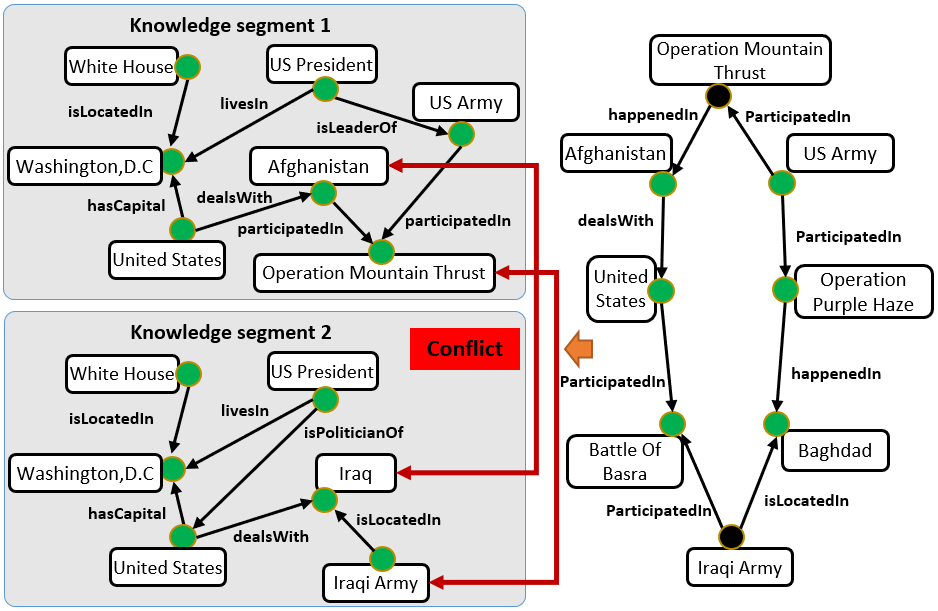
\includegraphics[width=0.47\textwidth]{img/iraq_operation.png}
	\caption{Pair-wise comparative reasoning results.}
	\label{iraq_inconsistency-example}
	\vspace{-1\baselineskip}
\end{figure}

\begin{figure}[]
	\centering
	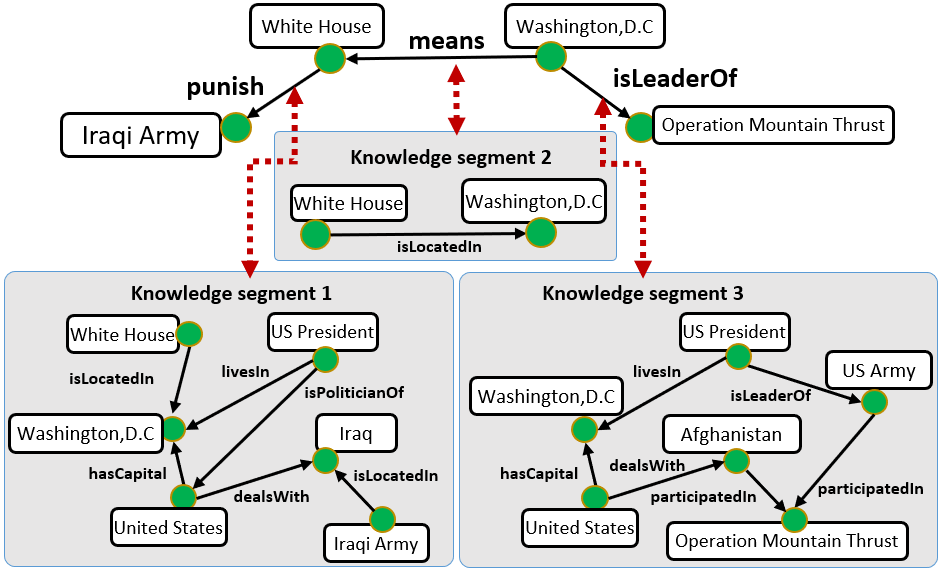
\includegraphics[width=0.47\textwidth]{img/iraq_collect.png}
	\caption{Collective comparative reasoning results.}
	\label{iraq_exp-coll}
	\vspace{-1\baselineskip}
\end{figure}
}



\vspace{-0.6\baselineskip}
\subsection{Collective Comparative Reasoning}\label{exp-coll-section}
\hide{
Here, we evaluate the effectiveness of the proposed collective comparative reasoning.
We test a query graph with three edges, including <{\tt White House}, {\tt punish}, {\tt Iraqi Army}>, <{\tt Washington,D.C}, {\tt means}, {\tt White House}> and <{\tt Washington,D.C}, {\tt participatedIn}, {\tt Operation Mountain Thrust}>.
Figure ~\ref{iraq_exp-coll} shows the query graph and the corresponding semantic matching subgraph.
As we can see, if we use the pair-wise comparative reasoning method to check each pair of them, all of them are true. %\footnote{For the query pair: <{\tt White House}, {\tt punish}, {\tt Iraqi Army}>, <{\tt Washington,D.C}, {\tt isLeaderOf}, {\tt Operation Mountain Thrust}>. Because these two clues have different subjects, so we won't check their inconsistency.}
However, if we use the collective comparative reasoning method, we could detect the inconsistency in the query graph as follows.

Table~\ref{iraq_coll-node-attr} and Table~\ref{iraq_coll-edge1} in Appendix show the node attribute influence, the node influence, and the edge influence of these three knowledge segments, respectively.
If we check each pair of clues in the query graph, we find that the key elements overlapping rate between $KS_1$ and $KS_3$ is more than 60\%. This is because the overlapping rates  are $66.6\%$ for node attribute influence, $100\%$ for node influence and $66.6\%$ for edge influence, which give the average overlapping rate $\frac{\frac{2}{3} + 1 + \frac{2}{3}}{3} = \frac{7}{9} > 60\%$.

Based on this, we future check <{\tt Washington,D.C}, {\tt isTypeOf}, {\tt White House}> or <{\tt White House}, {\tt isTypeOf}, {\tt Washington,D.C}>.
Our TF-IDF based predicate-predicate similarity between "{\tt isTypeOf}" and "{\tt isLocatedIn}" is 0.870. Thus, we have \textrm{infTrans}({\tt Washington,D.C}, {\tt White House}) $= 0.870 > 0.700$. This means that these two knowledge segments have the same subject. Finally, we check  <{\tt Operation Mountain Thrust}, {\tt isTypeOf}, {\tt Iraqi Army}> or <{\tt Iraqi Army}, {\tt isTypeOf}, {\tt Operation Mountain Thrust}>. According to the results in the previous subsection, we have that {\tt Iraqi Army} and {\tt Operation Mountain Thrust} are two different things. Therefore, we conclude that this query graph is inconsistent.

}


\begin{table}[!htbp]
	\centering
	\caption{Accuracy of collective comparative reasoning.}
	\fontsize{9}{9}\selectfont
	\setlength\tabcolsep{0.8pt}
	\begin{tabular}{|c|c|c|c|c|c|c|c|c|c|c|c|c|}
	\hline
	Dataset       & \makecell{\# of \\ queries}   & TransE & Jaccard  & KL  & KGMiner & Kompare \\ \hline
    Birth place positive   & 300     & 0.542 & 0.418 & 0.389 & 0.678 & \textbf{0.795} \\ \hline
    Birth place negative   & 300     & 0.465 & \textbf{0.996} & 0.968 & 0.970 & 0.829 \\ \hline
    Live place positive    & 300     & 0.448 & 0.451 & 0.465 & 0.635 & \textbf{0.989} \\ \hline
    Live place negative    & 300     & 0.558 & \textbf{1.000} & 0.860 & 0.924 & 0.743 \\ \hline
    Graduated college positive & 300  & 0.488 & 0.269 & 0.335 & 0.585 & \textbf{0.963} \\ \hline
    Graduated college negative & 300  & 0.545 & \textbf{0.996} & 0.928 & 0.907 & 0.829 \\ \hline

    $mean \pm std$ & - & 0.508 $\pm$ \textbf{0.045}  & 0.688 $\pm$ 0.313 & 0.658 $\pm$ 0.265 & 0.783 $\pm$ 0.155 & \textbf{0.858} $\pm$ 0.089  \\ \hline
    %Variance & - & \textbf{0.002} & 0.098 & 0.070 & 0.024 & 0.008  \\ \hline
	\end{tabular}
\label{coll_dataset}
\end{table}


We test collective comparative reasoning method on Yago dataset, using 6 query sets .
Different from the queries of pair-wise comparative reasoning which only contain two edges, each query of collective comparative reasoning contains 3 edges.
For example, in query set ``live Place", $<${\tt Barack Obama}, {\tt livesIn}, {\tt Washington,D.C.}$>$, $<${\tt Barack Obama}, {\tt is}, {\tt United States Senate Barack Obama}$>$ and $<${\tt United States Senate Barack Obama}, {\tt livesIn}, {\tt United States}$>$ is a positive query triad, while $<${\tt Barack Obama}, {\tt livesIn}, {\tt Washington,D.C.}$>$, $<${\tt Barack Obama}, {\tt is}, {\tt United States Senate Barack Obama}$>$ and $<${\tt United States Senate Barack Obama}, {\tt livesIn}, {\tt Canada}$>$ is an negative query triad.
The definition of the accuracy is the same as the previous section.
Following the setting of pair-wise reasoning, when checking the consistency of the query graph $<{\tt s_1}, {\tt p_1}, {\tt o_1}>$, $<{\tt s_1}, {\tt is}, {\tt s_2}>$ and $<{\tt s_2}, {\tt p_2}, {\tt o_2}>$,
we use baseline methods to check the truthness of this query triad, if any edge is classified as false, this query triad is treated as false. Otherwise,
we further check the truthness of $<{\tt o_1}, {\tt isTypeOf}, {\tt o_2}>$ and $<{\tt o_2}, {\tt isTypeOf}, {\tt o_1}>$,
if one of them is classified as true , this query pair is treated as consistency.
%\hh{double check: here you say 'if one of them is consistent/true' and in the covid19 paragraph (below), you say 'if any edge is ... false' which is which?}
Table ~\ref{coll_dataset} gives the detailed results.
As we can see, Jaccard ~\cite{jaccard} prefers to classify all queries as inconsistency and has the largest variance.
TransE ~\cite{transE} has the lowest variance, but its average accuracy is very low. \gchecker\ has the highest accuracy most of the time. It also has the highest average accuracy, and the second lowest variance.

%\subsection{Covid-19 Results}

\begin{table}[h]
	\centering
	\caption{Accuracy of collective comparative reasoning for Covid-19.}
	\fontsize{8}{9}\selectfont
	\setlength\tabcolsep{1.5pt}
	\begin{tabular}{|c|c|c|c|c|c|c|c|c|c|c|c|c|}
	\hline
	Dataset    & \# of queries      & TransE & Jaccard  & KL  & KGMiner & Kompare \\ \hline
    Positive    & 36    & 0.667 & 0.611 & \textbf{1.000} & 0.694 & \textbf{1.000} \\ \hline
    Negative    & 36    & 0.528 & 0.361 & 0.722 & 0.553 & \textbf{0.863} \\ \hline
    Average accuracy &  - & 0.598 $\pm$ 0.071  & 0.486 $\pm$ 0.126 & 0.861 $\pm$ 0.138 & 0.623 $\pm$ 0.071 & \textbf{0.932 $\pm$ 0.063}  \\ \hline
    %Variance & - & 0.005 & 0.016 & 0.019 & 0.005 & \textbf{0.004} \\ \hline
	\end{tabular}
\label{covid_coll}
\end{table}

We further provide experimental results on Covid-19 dataset.
We use queries which contain connections between drugs and genes/chemicals related to covid-19.\footnote{The query graphs can be found at \url{http://blender.cs.illinois.edu/covid19/visualization.html}.}
Among all these queries, we use queries which contain less than 8 nodes, and treat them as positive queries.
For each of the positive queries, we randomly select one node inside the query and substitute it with a randomly selected entity in the data graph, and treat the new query as the negative query.
%Following the setting of collective comparative reasoning,
For all the baseline methods, we use them to check all the edges inside the query, if any edge is classified as false, the whole query is treated as false.
Table ~\ref{covid_coll} shows the accuracy of different methods.
As we can see, \gchecker\ has the highest accuracy on both the positive and negative datasets, it also has the highest average accuracy and the lowest variance compared with other baseline methods.


\subsection{Efficiency Results}

%\hh{we need some efficiency results, e.g., runtime for ks extraction w.r.t. the kg size; runtime for comparative reasoning  w.r.t. the kg size; }
The runtime of knowledge segment extraction depends on the size of the underlying knowledge graphs. Among the two types of knowledge segments (edge-specific knowledge segment and subgraph-specific knowledge segment), subgraph-specific knowledge segment is most time-consuming. Figure ~\ref{fig:runtime}(a) shows that its runtime scales sub-linearly w.r.t. the number of nodes in the knowledge graph. Different lines show the runtime w.r.t. different query graph size.
Figure ~\ref{fig:runtime}(b) shows the runtime of comparative reasoning, where `Pair-wise' refers to the pairwise comparative reasoning, and the remaining bars are for collective comparative reasoning with $3$, $4$ and $5$ edges in the query graphs respectively. Note that the runtime of comparative reasoning only depends on the size of the the corresponding knowledge segments which typically have a few or a few tens of nodes. In other words, the runtime of comparative reasoning is {\em independent} of the knowledge graph size.


%%%%%+++++++++++++++++++++++++++++++++++
\begin{figure}\label{fig:runtime}
\vspace{-0.8\baselineskip}
\centering
%\hide{
%%%%% hspace is used to control the row and columns
%\subfloat[][Node-specific Knowledge Segment Extraction Runtime]{%
%\label{node-runtime}%
%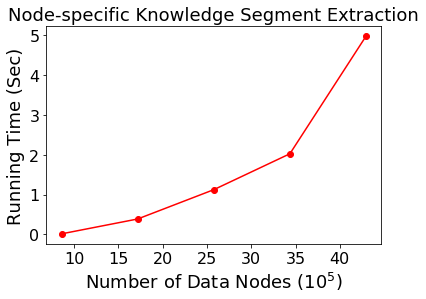
\includegraphics[height=1.7in]{img/node-specific-runtime.png}}%
%\hspace{50pt}%
%\subfloat[][Edge-specific Knowledge Segment Extraction Runtime]{%
%\label{edge-runtime}%
%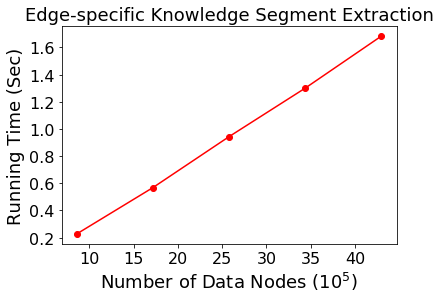
\includegraphics[height=1.7in]{img/edge-specific-runtime.png}}%
%}
%
%%\hspace{1pt}%
%\subfloat[h][Subgraph-specific KS extraction]{%
%\label{semantic-runtime-data}%
%\includegraphics[height=2in]{img/semantic-subgraph-data-time.png}}%
%%\hspace{50pt}%
%\subfloat[][Comparative reasoning]{%
%\label{comp-time}%
%\includegraphics[height=2in]{img/comparative-reasoning-runtime.png}}% \\
%%\hspace{1pt}%
	\begin{subfigure}[Subgraph-specific KS extraction]{
		\centering
		\includegraphics[width=0.45\textwidth]{submissions/logical-queries-uiuc/img/semantic-subgraph-data-time.png}
		\label{subfig:dbqa}}
	\end{subfigure}
	\begin{subfigure}[Comparative reasoning]{
		\centering
		\includegraphics[width=0.45\textwidth]{submissions/logical-queries-uiuc/img/comparative-reasoning-runtime.png}
		\label{subfig:dbqa}}
	\end{subfigure}
% \vspace{-1\baselineskip}
\caption[A set of four subfigures.]{
Runtime of \gchecker\
}
\label{precision-4}%
\label{fig:runtime}
\end{figure}
%%%%%+++++++++++++++++++++++++++++++++++



